\documentclass{article}
\usepackage{graphicx} % Required for inserting images
\usepackage{subcaption} % Para usar subfiguras, etc.
\usepackage[spanish]{babel} % Para que la fecha sea en español
\usepackage[colorlinks=true, linkcolor=blue, urlcolor=blue]{hyperref} % Para crear hipervínculos
\usepackage{wrapfig} % Texto al lado de una figura
\usepackage{multirow} % Permite juntar dos celas verticales de una tala
\usepackage{colortbl} % Permite colorear tablas
\usepackage[table]{xcolor} % Permite colorear una tabla de forma alterna

% Definición de colores
\definecolor{celeste}{RGB}{0, 255, 255}
\definecolor{gris}{RGB}{222, 222, 222} % Idóneo para alternar en las tablas

\graphicspath{{./images/}}

\title{Pruebas de latex}
\author{Carlos Vivero Barrera}

\begin{document}

\maketitle

\tableofcontents
\newpage

\section{Cosas varias}
    Nota de página\footnote{Heyyy}

    Palabras en \textbf{negrita}, \underline{subrayadas}, y en \textit{cursiva}
    \begin{center}
        Texto centrado
    \end{center}

    \large{Texto grande} vs \footnotesize{texto pequeño}
    
    Hipervínculo a la \hyperref[tab:tabla1]{tabla}
    \newpage

\section{Tablas}
% Tabla básica
    \begin{table}[h]
        \centering
        \begin{tabular}{|l|c|c|c|r|}
            \hline
            hol & hola & holaa & \multicolumn{2}{|c|}{holaaa} \\
            \hline
            \multirow[c]{2}{*}{0} & 1 & 2 & 3 & 4 \\
            \cline{2-5}
            & 1 & 2 & 3 & 4 \\
            \hline
        \end{tabular}
        \caption{Tabla de 3 x 5 básica}
        \label{tab:tabla1}
    \end{table}
    % Tablas coloreadas
    \begin{table}[h]
        \centering
        \label{tab:tabla2}
        \begin{subtable}{0.4\textwidth}
            \centering
            \label{tab:tabla2.1}
            \begin{tabular}{|c|c|c|c|}
                \hline
                \cellcolor{celeste}\textbf{Marca} & \cellcolor{celeste}\textbf{Modelo} & \cellcolor{celeste}\textbf{Precio} \\
                \hline
                \multirow[c]{2}{*}{Seat} & León & 8.000€ \\
                \cline{2-3}
                & Ibiza & 8.500€ \\
                \hline
                Mercedes & Benz & 12.000€ \\
                \hline
            \end{tabular}
            \caption{Tablas de coches}
        \end{subtable}
        \hfill
        \begin{subtable}{0.4\textwidth}
            \centering
            \label{tab:tabla2.2}
            \rowcolors{1}{white}{gris}
            \begin{tabular}{ c c c c c }
                \hline
                Número & \multicolumn{4}{ c }{Letras} \\
                \hline
                1 & a & b & c & d \\
                2 & e & f & g & h \\
                3 & i & j & k & l \\
                4 & m & n & ñ & o \\
                5 & p & q & r & s \\
                6 & t & u & v & w \\
                7 & x & y & z & :D \\
                \hline
            \end{tabular}
            \caption{Tabla coloreada de forma alterna}
        \end{subtable}
        \caption{Tablas de colores}
    \end{table}
    % Tabla coloreada de forma alterna
    
    \newpage

\section{Figuras}
    \subsection{Figura normal}
        \begin{figure}[ht] % La h hace que se coloque donde se llama, t para top y b para botom
            \centering
            
\includegraphics[scale=0.5]{./ElmoCines.png} % Poniendo solo esto también se muestra la imagen
            \caption{Esto es una figura de Elmo cines}
            \label{fig:Elmo cines}
        \end{figure}
    
    \subsection{Subfiguras}
        \begin{figure}[ht]
            \centering
            \begin{subfigure}{0.45\textwidth}
                \centering
                
\includegraphics[scale=0.5]{ElmoA.png}
                \caption{Esto es una figura de El}
                \label{fig:El}
            \end{subfigure}
            \hfill
            \begin{subfigure}{0.45\textwidth}
                \centering
                
\includegraphics[scale=0.5]{ElmoB.png}
                \caption{Esto es una figura de mo}
                \label{fig:mo}
            \end{subfigure} \\
            \begin{subfigure}{0.45\textwidth}
                \centering
                
\includegraphics[scale=0.5]{Elmo.png}
                \caption{Esto es una figura de Elmo}
                \label{fig:Elmo}
            \end{subfigure}
            %\caption{Esto son subfiguras}
            \label{fig:El-mo}
        \end{figure}
    
    \subsection{Texto al lado de figuras}
        \begin{wrapfigure}[6]{l}{0.3\linewidth}
            \vspace{-13pt}
            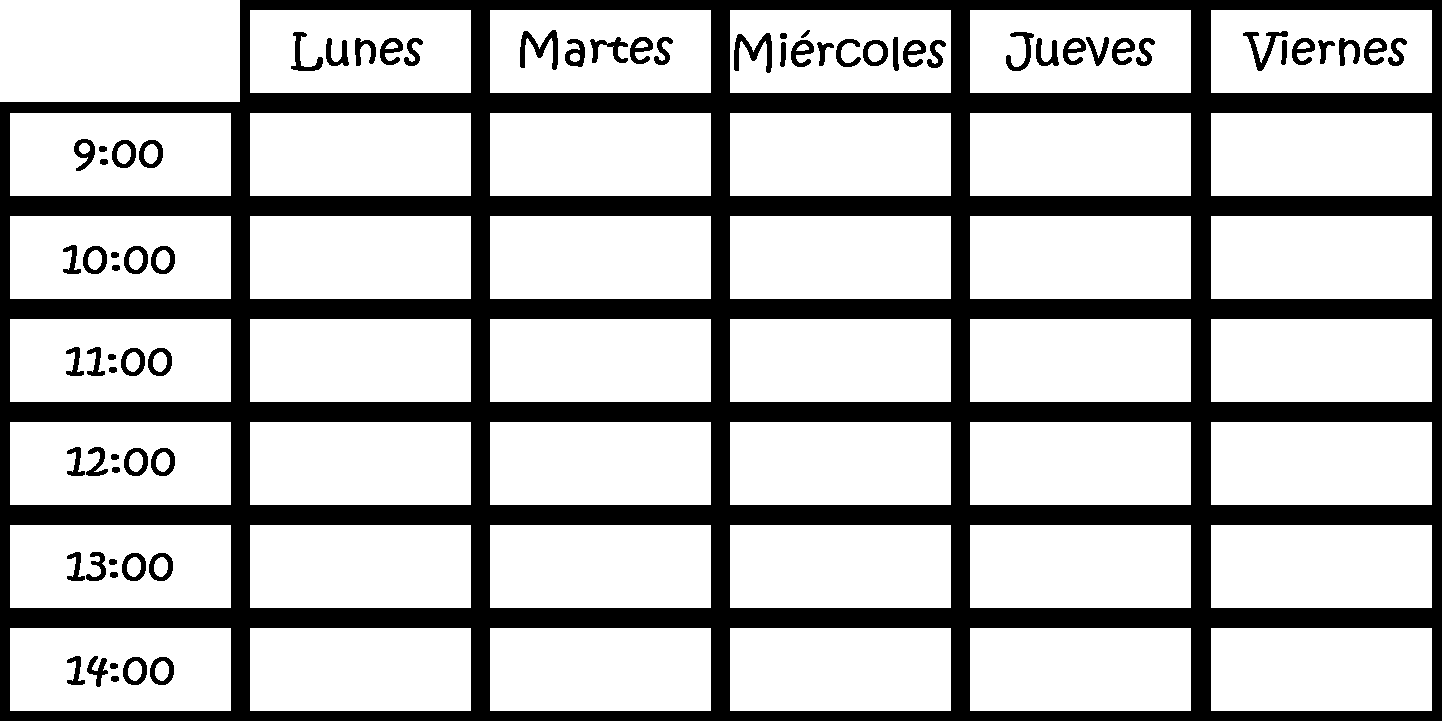
\includegraphics[scale=0.1]{PlantillaHorario.png}
        \end{wrapfigure}
        Esta es la plantilla de horario que utilizo todos los años con el paint
        para guardarme el nuevo horario en el móvil. Es simple, fácil, sencilla,
        maravillosa, espléndida, y muchísimos adjetivos más cuyo significado sea 
        algo bonito. Si estás interesado en tenerla, puedo ofrecerte una oferta
        por ella de 2.500€, nada mal en mi opinión por semejante obra de arte. A 
        todo esto, si te fijas la wrapfig ha cuadrado este texto perfectamente. 
        Una locura en mi humilde opinión.


\end{document}